% Signed Is Not Safe - IEEE conference-style paper (AI-ChainGuard, ESAIP Projet Applicatif 2)
% Build:  cd paper && pdflatex signed_is_not_safe.tex && pdflatex signed_is_not_safe.tex
% Figures and every quoted number: python paper/figures/make_figures.py (reads results/, writes figures/analysis.json)
\documentclass[conference]{IEEEtran}
\IEEEoverridecommandlockouts
\usepackage[utf8]{inputenc}
\usepackage[T1]{fontenc}
\usepackage{cite}
\usepackage{amsmath,amssymb}
\usepackage{graphicx}
\usepackage{booktabs}
\usepackage{array}
\usepackage{xurl}
\usepackage{xcolor}
\usepackage{tikz}
\usetikzlibrary{arrows.meta,positioning,fit}
\usepackage{dblfloatfix}
\usepackage{flushend}
\usepackage[hidelinks]{hyperref}
\hypersetup{pdftitle={Signed Is Not Safe: Measuring the Boundary Between Cryptographic Integrity and Semantic Trust in AI Supply Chains},pdfauthor={Karan Deshmukh, Sudheer Reddy Jogi, Dola Krishna Dama, Rambabu Mekala},pdfsubject={ESAIP MSc Cybersecurity and Data Science, Projet Applicatif 2}}
\newcommand{\sys}{AI-ChainGuard}
\newcommand{\st}[1]{\textsc{#1}}
\newcommand{\role}[1]{{\fontsize{4.5}{5}\selectfont\ttfamily #1}}

\begin{document}

\title{Signed Is Not Safe: Measuring the Boundary Between Cryptographic Integrity and Semantic Trust in AI Supply Chains}

\author{
\IEEEauthorblockN{Karan Deshmukh, Sudheer Reddy Jogi, Dola Krishna Dama, Rambabu Mekala}
\IEEEauthorblockA{MSc Cybersecurity and Data Science, ESAIP \'Ecole d'Ing\'enieurs, Angers, France\\
Projet Applicatif 2 (Applied AI Projects), supervised by Sofiane Hamrioui\\
Corresponding author: domail2karandeshmukh@gmail.com}
}

\maketitle

\begin{abstract}
A deployed model is the product of datasets, pretrained weights and fine-tuning steps that come from different parties, yet the controls that secure software supply chains sign one build or one file and say nothing about this lineage, nor about what a valid signature means for the behaviour of a model. We present \sys, a prototype that turns every artifact of an AI pipeline (dataset, base model, externally published model, fine-tuned model, deployment record) into a signed manifest whose payload embeds the manifest digests of its parents, giving a hash-linked provenance graph that a verifier checks with ten tests: bytes, row-level Merkle root, Ed25519 signature, role-bound signer policy, parent links, recursive ancestry, revocation, stage policy and content flags. Trust and revocation live in a signed, pinned, append-only log rather than in a database, and a deployment gateway verifies the whole chain once before loading a model from the verified bytes. We then \emph{measure} the boundary of such guarantees with a reproducible suite of 48 attack and control variants in seven experiments. Every manipulation made after signing is detected, from a $10^{-6}$ change to one weight and one trailing space in a dataset to a re-signed history rewrite, a rogue key written into the index and the truncation of the trust log, in 1.7--15.1\,ms including the chain. But a dataset poisoned \emph{before} signing verifies and deploys with a 77\,\% backdoor success rate behind a \st{verified} status, an adaptive trigger evades content heuristics at 51\,\%, and a trusted publisher's backdoored model verifies with 100\,\%. Attestation costs 0.8\,\% of training time, 8.5\,ms per full-chain verification, nothing per inference and 1.4--3.1\,KB per manifest; attestations export as in-toto statements in DSSE envelopes with ChainGuard or SLSA predicates. We argue that AI supply-chain controls must report cryptographic and semantic evidence separately, and release code, tests and scenarios.
\end{abstract}

\begin{IEEEkeywords}
AI supply chain, attestation, backdoor, data poisoning, digital signatures, in-toto, model provenance, revocation, SLSA, software supply chain security.
\end{IEEEkeywords}

\section{Introduction}
Machine-learning systems are assembled rather than written: a production model descends from a dataset collected by one team, a pretrained model downloaded from a public hub, a fine-tuning run on someone else's infrastructure and a packaging step, and every hand-over is an opportunity for substitution or manipulation. The incidents are real. In December 2022 a dependency-confusion attack replaced \texttt{torchtriton}, a dependency of the PyTorch nightly builds, by a package that exfiltrated SSH keys and files \cite{pytorch2022}. In February 2024 JFrog found about one hundred Hugging Face models whose pickle serialisation executed code on load, one opening a reverse shell \cite{jfrog2024}; in 2025 ReversingLabs described models whose deliberately broken pickle stream ran its payload before the scanner failed \cite{rl2025}. Poisoning is cheap: a 2025 study by Anthropic, the UK AI Security Institute and the Alan Turing Institute backdoored language models of 600\,M to 13\,B parameters with a near-constant 250 poisoned documents \cite{souly2025}, and Carlini \emph{et al.} poisoned web-scale datasets for tens of dollars \cite{carlini2024}. Article~15(5) of the EU AI Act now requires measures against ``attacks trying to manipulate the training data set (data poisoning), or pre-trained components used in training (model poisoning)'' \cite{aiact2024}; the NIST AI RMF \cite{nistairmf} and MITRE ATLAS technique AML.T0010, \emph{AI supply chain compromise} \cite{atlas}, frame the same risk.

The natural reaction is to reuse software supply-chain security: SLSA \cite{slsa11}, in-toto \cite{intoto2019} and Sigstore \cite{sigstore2022} give builds a verifiable provenance, and OpenSSF Model Signing extends Sigstore to model directories \cite{oms2025}. Two gaps remain. These tools attest a build or a file: nothing links the dataset to the base model, the base model to the fine-tuned model and that model to what was deployed, with a policy on who may sign which step and a revocation that propagates along the links. And a signature proves that bytes are what a key holder attested, yet users of model hubs are tempted to read \emph{signed} as \emph{safe}; for source code that reading is tolerable because code can be reviewed, for a tensor of weights it is not, and nobody has measured how far it is wrong.

This paper contributes (1)~\sys, an attestation chain across four pipeline stages with a recursive verifier of ten checks, a role-bound signer policy, a deployment gateway and a signed, pinned, append-only \emph{trust log} that removes the database from the trusted base for keys and revocations; (2)~a reproducible suite of 48 attack and control variants in seven experiments, from post-signing tampering and provenance rewriting to revocation bypasses against the log itself, untrusted publishers and poisoning before signing; (3)~a measurement of the boundary: every post-signing manipulation is detected, while signed poison verifies with a 77--100\,\% backdoor success rate and content heuristics are evaded; (4)~the cost of attestation and its interoperability through in-toto/DSSE and SLSA exports. Code, tests and scenarios are open source.\footnote{\url{https://github.com/domail2karandeshmukh-cyber/ai-chainguard}}

\section{Background and Related Work}\label{sec:related}

\subsection{Threats along an AI pipeline}
We distinguish threats by \emph{when} they act. After an artifact is signed, an attacker with access to storage, a mirror or the network can modify bytes, substitute an artifact, rewrite the recorded ancestry so that a model appears to descend from an approved dataset, forge or replay signatures, use a compromised or revoked key, or tamper with the system that records who is trusted and what is revoked; all of this is, in principle, within reach of cryptography. Before signing, an attacker who controls the data source, the publisher of a pretrained model or the training host plants a backdoor \cite{badnets} that a legitimate signer attests in good faith. Malicious serialisation \cite{jfrog2024,rl2025} sits in between: the file is exactly what was signed and executes code when loaded.

\subsection{Signing, provenance and transparency}
Sigstore replaces long-lived keys by short-lived certificates for OIDC identities (Fulcio) and records every signature in a public transparency log (Rekor) \cite{sigstore2022}. in-toto describes a supply chain as a layout of steps with authorised functionaries and verifies each step's link metadata \cite{intoto2019}; its attestation framework defines the \emph{Statement} (subject digests plus a typed predicate) and the DSSE envelope used by Sigstore and GitHub artifact attestations \cite{intotoattest,dsse}. SLSA v1.1 (April 2025) defines build-provenance levels and the provenance predicate consumed by policy engines \cite{slsa11}; OpenSSF Model Signing v1.0 (April 2025) hashes every file of a model directory into one signed manifest with Sigstore or PKI signatures \cite{oms2025}. The Update Framework pins a root role and protects against rollback with versioned, signed metadata \cite{tuf2010}; Certificate Transparency makes a log tamper-evident with a Merkle tree \cite{rfc6962}. Model cards \cite{modelcards} and datasheets \cite{datasheets} describe artifacts but are unsigned by default; safetensors removes code execution from loading \cite{safetensors}. Content defences such as Neural Cleanse \cite{neuralcleanse}, STRIP \cite{strip}, spectral signatures \cite{spectral} and activation clustering \cite{activation} detect some backdoors and are evadable by adaptive attackers. Table~\ref{tab:compare} positions \sys: it does not replace these tools; it links the artifacts they sign, enforces who may sign what, and reports what a signature does and does not establish.

\begin{table*}[t]
\caption{How \sys\ differs from existing approaches (capabilities as documented by each project, November 2026; ``no'' means not a goal of that tool). No column reaches ``yes'' for poisoned content: that is the boundary this paper measures.}
\label{tab:compare}
\centering
\scriptsize
\setlength{\tabcolsep}{4pt}
\begin{tabular}{@{}>{\raggedright}p{2.2cm}>{\raggedright}p{2.15cm}>{\raggedright}p{2.05cm}>{\raggedright}p{2.2cm}>{\raggedright}p{2.05cm}>{\raggedright}p{1.95cm}>{\raggedright\arraybackslash}p{2.85cm}@{}}
\toprule
 & Sigstore / cosign & OpenSSF Model Signing & in-toto layouts, SLSA provenance & Model cards, ML-BOM, registries (MLflow, DVC) & Backdoor scanners & \textbf{\sys} \\
\midrule
Scope & one artifact (OCI image, blob) & a model directory & steps of a software build & description, inventory, versions & model behaviour & \textbf{dataset $\to$ base $\to$ fine-tune $\to$ deployment} \\
Links stages & no & no & layout links steps; build inputs recorded & metadata lineage & no & \textbf{yes: parent manifest digests inside each signed payload} \\
Who may sign what & identity policies & signer identity & functionaries per step; builder identity & platform access control & n/a & \textbf{role per stage, verified (V4, V8); external publishers} \\
Revocation & certificate expiry, log & Sigstore ecosystem & key revocation in layout & stage transitions & n/a & \textbf{signed, pinned, append-only log; propagates to descendants} \\
Deployment decision & admission controllers & no & verification of the final product & no & no & \textbf{gateway: verify once, safe load, smoke test, signed record} \\
Poisoned content & no & no & no & no & partial, heuristic & partial: heuristics give \st{warning} only; \textbf{measured, not claimed} \\
\bottomrule
\end{tabular}
\end{table*}

\section{System Design}\label{sec:design}

\subsection{Threat model}
Trusted: the signing keys of the organisation, including the root key and the small pin file that anchors the trust log, the supply-chain policy and the verifier code. Treated as hostile: artifact storage, the index database, datasets, external model repositories, training hosts and the network. An attacker may read and write any artifact, manifest, index row or log record, replay or forge envelopes, hold a revoked key or publish models under an unknown identity. Out of scope are compromise of the trusted components, side channels, and the correctness of the training code. The verifier therefore recomputes every hash, digest and Merkle root instead of believing stored values, and reads nothing from the database that it could not confirm otherwise.

\begin{figure}[t]
\centering
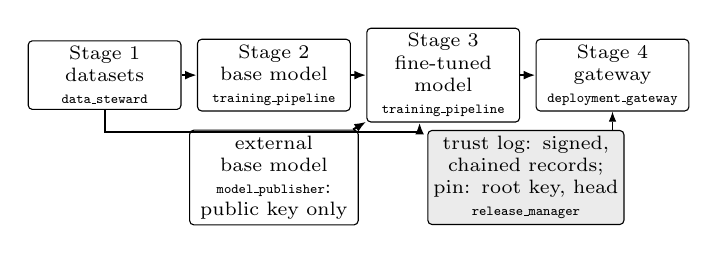
\begin{tikzpicture}[font=\scriptsize, x=1cm, y=1cm,
  box/.style={draw, rounded corners=1.5pt, align=center, inner sep=2pt, minimum height=7mm, text width=1.8cm},
  trust/.style={box, fill=black!8, text width=2.35cm},
  extb/.style={box, text width=2.0cm},
  arr/.style={-{Latex[length=1.5mm]}, thick},
  lnk/.style={-{Latex[length=1.3mm]}, densely dashed}]
\node[box] (ds) at (0,0) {Stage 1\\datasets\\\role{data\_steward}};
\node[box] (bm) at (2.15,0) {Stage 2\\base model\\\role{training\_pipeline}};
\node[box] (ft) at (4.3,0) {Stage 3\\fine-tuned model\\\role{training\_pipeline}};
\node[box] (gw) at (6.45,0) {Stage 4\\gateway\\\role{deployment\_gateway}};
\node[extb] (ext) at (2.15,-1.3) {external base model\\\role{model\_publisher}: public key only};
\node[trust] (log) at (5.35,-1.3) {trust log: signed, chained records; pin: root key, head\\\role{release\_manager}};
\draw[arr] (ds) -- (bm);
\draw[arr] (bm) -- (ft);
\draw[arr] (ft) -- (gw);
\draw[arr] (ext) -- (ft);
\draw[arr] (ds.south) -- ++(0,-0.28) -| ([xshift=-3mm]ft.south);
\draw[lnk] (log.north -| gw.south) -- (gw.south);
\end{tikzpicture}
\caption{Four attested stages and the signing role of each. Each child's signed payload embeds the manifest digests of its parents (solid arrows). Internal base models require a dataset parent; an external base model has no internal lineage and may be signed only by a registered publisher key. The gateway re-verifies the whole chain, and every verification replays the signed trust log (dashed).}
\label{fig:arch}
\end{figure}

\subsection{Manifests and the hash-linked chain}
Every artifact receives a manifest body $m$: its type and pipeline stage, the SHA-256 and size of the file, for CSV datasets the Merkle root over the hashes of its rows, the list of parents, free-form provenance (training configuration, environment), the results of pre-attestation content checks, and the signer's identity, role and key id. The body is serialised in a canonical JSON form (sorted keys, no insignificant whitespace) and signed as a whole with Ed25519 \cite{rfc8032}:
\begin{equation}
\sigma = \mathrm{Sign}_{k}\bigl(\mathrm{canon}(m)\bigr),\qquad
d(m) = \mathrm{SHA256}\bigl(\mathrm{canon}(m)\bigr).
\label{eq:sign}
\end{equation}
Signing the whole body rather than the file hash alone prevents an attacker from keeping a valid (hash, signature) pair and changing the stage, the parents or the signer role around it. The manifest digest $d(m)$ is the artifact's identity in the provenance graph: a child lists each parent as $(\mathrm{id}_p, d(m_p), \mathrm{relation})$ inside its own signed body, so that
\begin{equation}
d(m_{\mathrm{child}}) \text{ commits to } d(m_p) \text{ for every ancestor } p,
\label{eq:chain}
\end{equation}
as a Git commit commits to its parents. Rewriting an ancestor, even re-signing it with the legitimate key, changes $d(m_p)$ and breaks every descendant. For datasets, the Merkle tree (RFC~6962 construction over line hashes) lets the verifier report \emph{which} rows changed, authenticated by the signed root; the leaf hashes are kept in a sidecar that is trusted only if it reproduces that root.

\subsection{Verification: ten checks and three outcomes}
Verification of an artifact runs ten checks and recurses into its parents (Table~\ref{tab:checks}). The outcome is derived, never set: \st{failed} if any check fails, \st{warning} if integrity holds but a content check flagged the data here or upstream, \st{verified} otherwise. \st{verified} means \emph{exactly what trusted, unrevoked signers in authorised roles attested, through an intact ancestry}; the system never upgrades it to ``safe''. The policy file states which role may sign which stage and which parent types each stage requires or forbids: an internal base model must descend from a dataset, a fine-tuned model from a dataset and exactly one base model of either kind, and the training key may not sign the external-import stage, so an internal model cannot be relabelled ``external'' to escape the dataset rule. Every report also records the sequence number and head hash of the trust log it was verified against, and names the external artifacts whose provenance ends at a publisher.

\begin{table}[t]
\caption{The ten checks of a verification}
\label{tab:checks}
\centering
\scriptsize
\setlength{\tabcolsep}{3pt}
\begin{tabular}{@{}l>{\raggedright}p{2.05cm}>{\raggedright\arraybackslash}p{4.75cm}@{}}
\toprule
 & Check & Fails when \\
\midrule
V0 & Envelope & missing, malformed, or swapped (stored under another id) \\
V1 & File hash & SHA-256 or size differs from the signed values \\
V2 & Dataset Merkle root & rows changed (the report lists which lines) \\
V3 & Ed25519 signature & invalid over the canonical body, or key not in the signed trust log \\
V4 & Signer trust & key revoked, role or identity mismatch, role not allowed for the stage, index and log disagree \\
V5 & Parent links & a parent envelope is missing or its recomputed digest differs from the embedded one \\
V6 & Ancestry & any ancestor \st{failed} (recursive) \\
V7 & Revocation & artifact or ancestor revoked in the signed log, index row deleted, or index flag cleared against the log \\
V8 & Policy & wrong type for stage, missing or forbidden parent types, parent from a later stage \\
V9 & Content flags & a signed pre-attestation content check flagged the data here or upstream: \st{warning} only \\
\bottomrule
\end{tabular}
\end{table}

\subsection{The signed trust log}
Until the previous version the trust store (which public key belongs to which identity and role) and the revocation flags lived in the SQLite index, and our own revocation experiment showed the consequence: an attacker able to write that file could clear a \texttt{revoked} flag and the withdrawn model verified again. Trust and revocation are now records of an append-only log. Record $i$ carries a sequence number, the hash of record $i-1$, a timestamp, an action (\texttt{trust\_key}, \texttt{revoke\_key}, \texttt{revoke\_artifact}, \texttt{rotate\_root}) and its subject, and is signed by the root key $k_R$ of the \texttt{release\_manager} role:
\begin{align}
r_i &= \bigl(e_i,\ \mathrm{Sign}_{k_R}(\mathrm{canon}(e_i))\bigr),\qquad h_{i-1}\in e_i, \label{eq:log}\\
h_i &= \mathrm{SHA256}\bigl(\mathrm{canon}(r_i)\bigr). \nonumber
\end{align}
A pin file in the trusted keys directory holds the root public key and the pair $(n, h_n)$ of the last record. The verifier replays the log at every verification: each signature must verify under the active root (a \texttt{rotate\_root} record signed by the old root introduces a new one), each record must chain to the previous, and the log must end exactly at the pinned head. A truncated log (rollback), an edited record, a deleted or substituted log, or a key present in the index but absent from the log, all make V3, V4 and V7 fail closed, and an index that disagrees with the log is reported as tampering. The structure is a single-writer transparency log without a Merkle tree, since it is small, with TUF-style root pinning and rollback protection \cite{tuf2010}; publishing the records to a shared log such as Rekor so that all verifiers see one history is the natural next step. There is no un-revoke action: a withdrawn artifact is replaced by a new version.

\subsection{Deployment gateway and external publishers}
The gateway is the last line of defence. It verifies the full chain once, refuses a \st{failed} model and, by default, a \st{warning} one, refuses pickle-based formats, reads the model bytes once, re-hashes them and loads the model from those same bytes so that there is no time-of-check/time-of-use gap, runs a smoke test on held-out data, computes a release root (the Merkle root over the manifest digests of the model and its ancestors) and signs a deployment record that also binds the trust-log head it verified against. Inference then runs on the loaded model without further verification. A model from an outside publisher enters through a separate path: the publisher signs a manifest with its own key, an administrator registers the publisher's \emph{public} key out of band, and the import refuses anything unsigned or structurally wrong, stores the rest and verifies it; a failed import is kept as quarantined evidence that cannot be used as a parent or deployed. Its provenance ends, by design, at the publisher's identity.

\subsection{Interoperability}
Any attestation exports as an in-toto Statement v1 inside a DSSE envelope \cite{intotoattest,dsse}, signed over the pre-authentication encoding with the role key that signed the original manifest, with either a ChainGuard predicate (the full manifest) or a SLSA Provenance v1 predicate \cite{slsa11} in which the training or fine-tuning stage is the build, the dataset and base model are resolved dependencies, the signing role is the builder and the manifest digest and Merkle root travel as by-products. The export is verified by an independent DSSE verifier in the test suite, including the specification's PAE test vector.

\section{Implementation}\label{sec:impl}
\sys\ is about 8\,200 lines of Python 3.11+ (PyTorch, scikit-learn, \texttt{cryptography}, FastAPI, Streamlit) plus 1\,600 lines of tests; one core library holds all security logic, and the CLI, REST API, ML pipeline, gateway, attack scenarios and CI are thin consumers of it. Private keys are PKCS\#8 files with owner-only permissions or CI secrets, the index is SQLite, and the JSON envelopes on disk are the source of truth. The reference pipeline exports the scikit-learn digits dataset (8$\times$8 images; 1\,000 training, 437 fine-tuning, 360 held-out samples), attests the datasets with content checks (label distribution against a reference, duplicate rows, a known trigger pattern), trains a 38\,282-parameter CNN, fine-tunes it and sends it through the gateway. A dashboard exposes verification, provenance, an attack lab, external models, the trust log with sandboxed bypass attempts, metrics and events, and can embed the API for one-container deployments; Docker Compose and GitHub Actions workflows are provided. \emph{Reproducibility:} 168 automated tests run in 36\,s; \texttt{attacks/run\_all.py} regenerates every table, \texttt{scripts/benchmark.py} every cost figure, and \texttt{paper/figures/make\_figures.py} writes every number quoted below to \texttt{analysis.json}.

\section{Evaluation}\label{sec:eval}

\subsection{Setup and protocol}
All numbers come from one run on 9~November 2026 in the reference development environment, a cloud Linux container with two logical Intel Xeon cores at 2.10\,GHz, 8\,GB of memory and no GPU (Python 3.13, PyTorch 2.15 on CPU). Each attack variant starts from a fresh copy of a clean, fully attested chain, applies one manipulation as an attacker with the corresponding access would, verifies the targeted artifact with its whole chain and records the outcome, the checks that fired and the wall time of that verification; a variant is correct when the observed outcome equals the predicted one, and untouched controls must stay \st{verified}. Backdoor experiments train real models: the poison is a BadNets-style 2$\times$2 corner patch \cite{badnets} applied to 8\,\% of the training rows with the label changed to~7, and the attack success rate (ASR) is the share of held-out images that carry the trigger and are classified as~7. The containerised pipeline (\st{verified}$\to$\st{deployed}, clean accuracy 0.950), API and dashboard were also executed on a team laptop (MacBook Air) on 16~October 2026; tests and benchmarks have not yet been repeated there.

\subsection{Post-signing attacks are detected}
Table~\ref{tab:suite} summarises the seven experiments; Fig.~\ref{fig:det}(a) shows every variant. All 48 variants ended with the predicted outcome. Every manipulation made after signing was rejected, including the subtle ones: flipping the labels of five rows, appending one row or adding a single trailing space to a signed dataset (V1, V2, with the changed lines named), nudging one weight by $10^{-6}$ or re-saving identical weights in another format (V1), deleting a parent record, re-signing a modified parent with the legitimate key, editing a parent link without re-signing or presenting a model with no dataset ancestry (V5, V3, V8), and corrupting, replaying, mis-roling or signing with unknown or revoked keys (V3, V4). Revocation of an artifact or a key fails every descendant and blocks deployment, while a dataset signed by another role still verifies after a training-key revocation, so the blast radius is the key's. Detection, measured as the verification time of the attacked artifact with its chain, took 1.7--15.1\,ms (median 7.5\,ms).

\begin{table}[t]
\caption{The attack suite: 48 variants, all with the predicted outcome. Checks: the ones that fired on attacks of that experiment.}
\label{tab:suite}
\centering
\scriptsize
\setlength{\tabcolsep}{2.5pt}
\begin{tabular}{@{}c>{\raggedright}p{2.45cm}c>{\raggedright}p{2.6cm}>{\raggedright\arraybackslash}p{1.05cm}@{}}
\toprule
Exp. & Experiment (scenario) & Var. & Outcome & Checks \\
\midrule
1 & Dataset tampering (A) & 5 & control \st{verified}; 4 \st{failed} & V1, V2, V6 \\
2 & Model substitution (B) & 4 & control \st{verified}; 3 \st{failed} & V1 \\
3 & Invalid signature, key misuse (D) & 7 & control \st{verified}; 6 \st{failed} & V3, V4, V6 \\
4 & Broken provenance (C) & 5 & control \st{verified}; 4 \st{failed} & V3, V5, V8 \\
5 & Revocation and 8 bypasses (F) & 13 & 2 \st{verified} as predicted; 11 \st{failed}, gateway blocks & V3, V4, V6, V7 \\
6 & Poison before signing (E) & 5 & E1 \st{failed}; E3 \st{warning}; E2, E4 \st{verified} (Fig.~\ref{fig:boundary}) & V6, V9 \\
7 & Untrusted external source (G) & 9 & 3 \st{verified}; 4 \st{failed}; 2 \st{refused} at import & V1, V3, V4, V6 \\
\bottomrule
\end{tabular}
\end{table}

\subsection{Attacks on the trust itself}
Experiment~5 targets the mechanisms that decide who is trusted: after a base model is revoked, eight bypasses try to make its fine-tuned descendant verify again. Editing the index (deleting the revoked artifact's row, C1; deleting the revoked key, C2; overwriting the cached status, C3) already failed in the previous version, because the verifier never reads a cached status and treats a missing row as unknowable revocation. Clearing the \texttt{revoked} flag (C4) was that version's documented limitation and now fails: the signed log still says revoked, and the disagreement raises an \texttt{INDEX\_TAMPERING} event (V6, V7). A rogue key written into the index with the training role and used to re-sign a substituted model (C5) fails because the key never entered the signed log (V3, V4). Truncating the log to drop the revocation (C6), editing the record in place (C7) and deleting the log (C8) fail closed (V3, V4, V6, V7): the replay no longer ends at the pinned head or no longer verifies under the root key. What remains trusted is the keys directory: whoever holds the root key and can rewrite the pin controls the trust decisions, as the threat model states.


\subsection{Signed is not safe}
Experiments~6 and~7 measure what the signature does not cover (Fig.~\ref{fig:boundary}). The clean pipeline (E0) deploys a model with 95.0\,\% clean accuracy and 0\,\% ASR. Poison injected into the signed dataset \emph{after} signing (E1) fails the chain at V6, as expected. When the data steward signs a dataset poisoned \emph{before} attestation (E2), every check passes: the fine-tuned model deploys as \st{verified} with 94.2\,\% clean accuracy, indistinguishable from the clean model on ordinary inputs, and a 77.2\,\% ASR. With pre-attestation content checks (E3) the known corner trigger is flagged, the dataset carries a signed flag, the model verifies with \st{warning} and the gateway blocks it by default: heuristics work as evidence. An adaptive attacker who moves the trigger to a pattern the checks do not know (E4) deploys as \st{verified} with 51.2\,\% ASR. Experiment~7 repeats the lesson at the supply-chain boundary: a backdoored model trained by a \emph{trusted}, registered publisher imports as \st{verified} with 93.3\,\% clean accuracy and a 100\,\% ASR, while the unknown publisher, the model modified in transit, the unsigned model and the revoked publisher key are all rejected (Table~\ref{tab:suite}). A valid signature proves \emph{who} attested and \emph{that nothing changed since}; it transfers trust to the signer and creates none.

\begin{figure}[t]
\centering
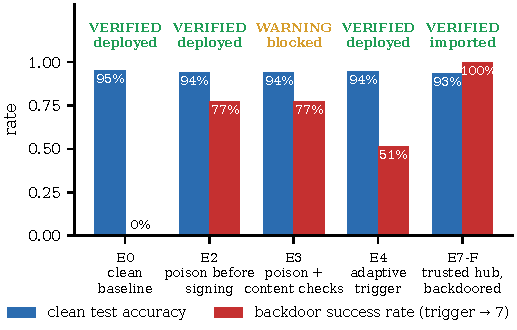
\includegraphics[width=0.94\columnwidth]{figures/fig_boundary.pdf}
\caption{Experiments 6 and 7: clean accuracy and backdoor success rate of the deployed or imported model, with its verification status. Signed poison (E2) and a trusted publisher's backdoor (E7-F) pass every cryptographic check; content checks catch a known trigger (E3) and miss an adaptive one (E4).}
\label{fig:boundary}
\end{figure}

\begin{figure*}[t]
\centering
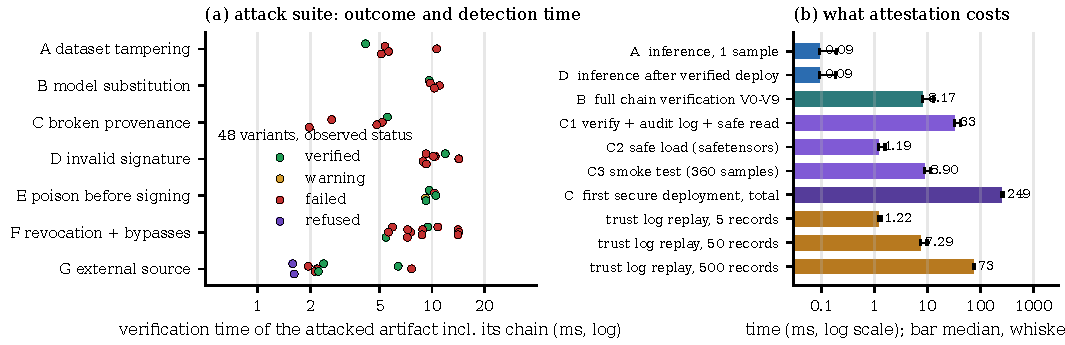
\includegraphics[width=0.93\textwidth]{figures/fig_detection_cost.pdf}
\caption{(a) Outcome and verification time of all 48 variants, grouped by scenario (fresh chain per variant; the time includes the whole ancestry and the trust-log replay). (b) The cost of attestation in the reference environment: inference before and after a verified deployment, full-chain verification, the components of the first secure deployment, and the replay of trust logs of 5, 50 and 500 records with every signature verified.}
\label{fig:det}
\end{figure*}

\subsection{Cost}
Fig.~\ref{fig:det}(b) gives the cost. Attesting the four artifacts of the pipeline took 10.7\,ms against 1\,288\,ms of training (0.83\,\%; the share is workload-dependent and shrinks for larger models). A full chain verification of the fine-tuned model with its three ancestors takes 8.5\,ms (median of 200 runs; p95 12.2\,ms); replaying the 5-record trust log accounts for 0.16\,ms of it (0.75\,ms cold). The first secure deployment costs 253\,ms once, dominated by audit-trail writes (31\,ms) and a second chain verification when the deployment record is registered (safe load 1.1\,ms, smoke test 8.3\,ms). A prediction then costs 0.084\,ms before and 0.085\,ms after the verified deployment: verification is not on the inference path. Signed envelopes are 1.4--3.1\,KB per artifact; the row-level Merkle sidecar of a dataset is linear in its rows (30 and 68\,KB here; one million rows hash in 1.7\,s). SHA-256 runs at about 1.2\,GB/s, so a 256\,MiB model hashes in 220\,ms; Ed25519 signing (0.04\,ms) and verification (0.12--0.14\,ms) do not depend on size. Replaying the trust log costs about 0.14\,ms per record when every signature is verified (0.8, 6.9, 69 and 288\,ms for 5, 50, 500 and 2\,000 records; 0.8\,MB for the largest) and 15\,$\mu$s per record once signatures are cached within a process; an organisation with thousands of records would checkpoint a signed snapshot rather than replay from genesis.

\section{Discussion and Limitations}\label{sec:discussion}
The measurements are an upper bound on what the design offers. The attack suite is written by the defenders and runs on an 8$\times$8-digit CNN: it shows that the cryptographic checks behave as designed and how large the semantic gap is on a small model, not that the gap has that size for a language model, where poisoning is cheaper \cite{souly2025}. The content checks are simple heuristics chosen to show that heuristics can be evaded (E4); stronger defences \cite{neuralcleanse,strip,spectral,activation} would raise the bar without closing it. Trust rests on long-lived Ed25519 keys in files: a stolen, unrevoked key signs valid manifests, which argues for short-lived keyless certificates \cite{sigstore2022} and hardware-backed keys. The trust log is local and single-writer, so a verifier holding a stale copy would miss a recent revocation, and the pin file is as critical as the root key. The canonical JSON is Python-only rather than RFC~8785 \cite{rfc8785}, the API has no authentication, the gateway verifies the chain twice on a first deployment, and tests and benchmarks have run in one environment. None of this touches the central result, which holds by construction: signatures are evidence about origin and integrity, and a report that shows \st{verified} without saying so invites the wrong conclusion. \sys\ therefore keeps cryptographic and content evidence in separate checks (V0--V8 versus V9), labels external provenance that ends at a publisher, and never lets a heuristic produce a \st{failed} or a signature produce a ``safe''.

\section{Conclusion}
We built an attestation chain for AI pipelines that links datasets, base models, externally published models, fine-tuned models and deployments through signed manifests that embed their parents' digests, enforces who may sign which stage, keeps trust and revocation in a signed, pinned, append-only log, and gates deployment on a full-chain verification. On 48 attack and control variants every manipulation made after signing was detected, including bypasses aimed at the index and at the log itself, at a cost of under one per cent of training time, 8.5\,ms per verification and nothing per inference. The same suite shows the limit: poison present before signing verifies and deploys with a 77\,\% backdoor success rate, and a trusted publisher's backdoor with 100\,\%. AI supply-chain security needs both kinds of evidence, reported separately; this prototype provides the first kind and measures where the second must take over. Next steps are the publication of the trust log to a shared transparency log, keyless signing for the roles, reproduction on team hardware and larger models.

\section*{Acknowledgment}
The authors thank Sofiane Hamrioui, ESAIP Angers, for supervising this project. The prototype was developed with AI-assisted code generation and validated by execution; the team is responsible for its design, evaluation and conclusions.

\begin{thebibliography}{00}
\bibitem{pytorch2022} PyTorch team, ``Compromised PyTorch-nightly dependency chain between December 25th and December 30th, 2022,'' Dec. 31, 2022. [Online]. Available: \url{https://pytorch.org/blog/compromised-nightly-dependency/}
\bibitem{jfrog2024} D. Cohen, JFrog Security Research, ``Data scientists targeted by malicious Hugging Face ML models with silent backdoor,'' Feb. 2024. [Online]. Available: \url{https://jfrog.com/blog/data-scientists-targeted-by-malicious-hugging-face-ml-models-with-silent-backdoor/}
\bibitem{rl2025} K. Zanki, ReversingLabs, ``Malicious ML models discovered on Hugging Face platform,'' Feb. 2025. [Online]. Available: \url{https://www.reversinglabs.com/blog/rl-identifies-malware-ml-model-hosted-on-hugging-face}
\bibitem{souly2025} A. Souly, J. Rando, E. Chapman, X. Davies, B. Hasircioglu, E. Shereen, C. Mougan, V. Mavroudis, E. Jones, C. Hicks, N. Carlini, Y. Gal, and R. Kirk, ``Poisoning attacks on LLMs require a near-constant number of poison samples,'' arXiv:2510.07192 [cs.CR], Oct. 2025.
\bibitem{carlini2024} N. Carlini, M. Jagielski, C. A. Choquette-Choo, D. Paleka, W. Pearce, H. Anderson, A. Terzis, K. Thomas, and F. Tram\`er, ``Poisoning web-scale training datasets is practical,'' in \emph{Proc. IEEE Symp. Security and Privacy (SP)}, 2024, pp. 407--425.
\bibitem{aiact2024} European Parliament and Council, ``Regulation (EU) 2024/1689 of 13 June 2024 laying down harmonised rules on artificial intelligence (Artificial Intelligence Act),'' \emph{Off. J. Eur. Union}, L, 2024/1689, 12 Jul. 2024, Art. 15(5).
\bibitem{nistairmf} NIST, ``Artificial Intelligence Risk Management Framework (AI RMF 1.0),'' NIST AI 100-1, Jan. 2023.
\bibitem{atlas} MITRE, ``ATLAS technique AML.T0010: AI supply chain compromise.'' [Online]. Available: \url{https://atlas.mitre.org/techniques/AML.T0010}
\bibitem{slsa11} OpenSSF, ``SLSA specification v1.1: Supply-chain Levels for Software Artifacts,'' Apr. 2025. [Online]. Available: \url{https://slsa.dev/spec/v1.1/}
\bibitem{intoto2019} S. Torres-Arias, H. Afzali, T. K. Kuppusamy, R. Curtmola, and J. Cappos, ``in-toto: Providing farm-to-table guarantees for bits and bytes,'' in \emph{Proc. 28th USENIX Security Symp.}, 2019, pp. 1393--1410.
\bibitem{sigstore2022} Z. Newman, J. S. Meyers, and S. Torres-Arias, ``Sigstore: Software signing for everybody,'' in \emph{Proc. ACM SIGSAC Conf. Computer and Communications Security (CCS)}, 2022, pp. 2353--2367.
\bibitem{oms2025} OpenSSF, Sigstore, NVIDIA, and HiddenLayer, ``OpenSSF Model Signing (OMS) specification v1.0'' and the \texttt{model-signing} reference implementation, Apr. 2025. [Online]. Available: \url{https://github.com/sigstore/model-transparency}
\bibitem{intotoattest} in-toto project, ``in-toto Attestation Framework: Statement v1.'' [Online]. Available: \url{https://github.com/in-toto/attestation}
\bibitem{dsse} Secure Systems Lab, ``DSSE: Dead Simple Signing Envelope, protocol v1.'' [Online]. Available: \url{https://github.com/secure-systems-lab/dsse}
\bibitem{tuf2010} J. Samuel, N. Mathewson, J. Cappos, and R. Dingledine, ``Survivable key compromise in software update systems,'' in \emph{Proc. ACM Conf. Computer and Communications Security (CCS)}, 2010, pp. 61--72.
\bibitem{rfc6962} B. Laurie, A. Langley, and E. Kasper, ``Certificate Transparency,'' RFC 6962, IETF, Jun. 2013.
\bibitem{rfc8032} S. Josefsson and I. Liusvaara, ``Edwards-Curve Digital Signature Algorithm (EdDSA),'' RFC 8032, IETF, Jan. 2017.
\bibitem{rfc8785} A. Rundgren, B. Jordan, and S. Erdtman, ``JSON Canonicalization Scheme (JCS),'' RFC 8785, IETF, Jun. 2020.
\bibitem{badnets} T. Gu, B. Dolan-Gavitt, and S. Garg, ``BadNets: Identifying vulnerabilities in the machine learning model supply chain,'' arXiv:1708.06733 [cs.CR], 2017.
\bibitem{modelcards} M. Mitchell, S. Wu, A. Zaldivar, P. Barnes, L. Vasserman, B. Hutchinson, E. Spitzer, I. D. Raji, and T. Gebru, ``Model cards for model reporting,'' in \emph{Proc. Conf. Fairness, Accountability, and Transparency (FAT*)}, 2019, pp. 220--229.
\bibitem{datasheets} T. Gebru, J. Morgenstern, B. Vecchione, J. W. Vaughan, H. Wallach, H. Daum\'e III, and K. Crawford, ``Datasheets for datasets,'' \emph{Commun. ACM}, vol. 64, no. 12, pp. 86--92, 2021.
\bibitem{safetensors} Hugging Face, ``Safetensors: a simple, safe way to store and distribute tensors,'' documentation; security audit by Trail of Bits, 2023. [Online]. Available: \url{https://huggingface.co/docs/safetensors}
\bibitem{neuralcleanse} B. Wang, Y. Yao, S. Shan, H. Li, B. Viswanath, H. Zheng, and B. Y. Zhao, ``Neural Cleanse: Identifying and mitigating backdoor attacks in neural networks,'' in \emph{Proc. IEEE Symp. Security and Privacy (SP)}, 2019, pp. 707--723.
\bibitem{strip} Y. Gao, C. Xu, D. Wang, S. Chen, D. C. Ranasinghe, and S. Nepal, ``STRIP: A defence against trojan attacks on deep neural networks,'' in \emph{Proc. Annu. Computer Security Applications Conf. (ACSAC)}, 2019, pp. 113--125.
\bibitem{spectral} B. Tran, J. Li, and A. Madry, ``Spectral signatures in backdoor attacks,'' in \emph{Advances in Neural Information Processing Systems (NeurIPS)}, 2018, pp. 8011--8021.
\bibitem{activation} B. Chen, W. Carvalho, N. Baracaldo, H. Ludwig, B. Edwards, T. Lee, I. Molloy, and B. Srivastava, ``Detecting backdoor attacks on deep neural networks by activation clustering,'' in \emph{Proc. AAAI Workshop on Artificial Intelligence Safety (SafeAI)}, 2019.
\end{thebibliography}

\end{document}
